\section{Fase di Download}
\subsection{Descrizione}
Il trasferimento dati da un peer ad un altro è il cuore dell'applicazione. Dopo infatti la fase di registrazione e quella di ricerca di un determinato file, un peer può finalmente contattare l'indirizzo specifico di chi lo possiede (sempre nel caso in cui almeno un peer nella rete abbia il file da condividere).
\subsection{Struttura}
Ogni peer mantiene una socket TCP attiva in ascolto, pronto a ricevere una richiesta di trasferimento dati e avviare l'upload del file richiesto. \linebreak
Tramite la configurazione del file config, è possibile impostare il numero massimo di upload che ogni nodo puo avviare contemporaneamente. Per quanto riguarda il download invece, è possibile effetuarne solo uno alla volta ed anche la ricezione del file avviene da un unico indirizzo IP specifico.
\linebreak
\linebreak
I dati da inviare vengono suddivisi in pacchetti di dimensione prefissata (512 byte) detti CHUNK: questa struttura consente sia di avere una sicurezza ulteriore nel download ( un file molto grande inviato per intero avrebbe piu possibilità di essere ricevuto corrotto) sia di poter riprendere il download nel caso in cui il trasferimento sia stato interrotto per un qualche motivo. Il peer infatti potrebbe richiedere il file dall'ultimo CHUNK ricevuto senza ricominciare il download dall'inizio.\linebreak
La fase di download è "bloccante": l'utente non puo effettuare altre operazioni una volta che ha digitato il comando per avviare il trasferimento dei dati; l'unico segnale che continua a rimanere attivo è il ping inviato periodicamente al superpeer.\linebreak
\linebreak
L'applicazione richiede che ogni peer metta a disposizione due cartelle diverse, una per i file da condividere (cartella\_condivisa; impostabile nel file di configurazione) ed una per i file scaricati (Scaricati; non impostabile). Questa distinzione nasce dal fatto di voler evitare che un peer cominci a condividere un oggetto che lui stesso sta scaricando da un'altra fonte, ma che non è ancora completo (la verifica infatti che un file sia disponibile ad essere inviato viene fatta sulla presenza del nome del file in cartella\_condivisa).
\subsection{Esempio di esecuzione}
Si consideri il caso in cui ci siano due peer, A e B, e il primo voglia scaricare un file dal secondo. La funzione di download implementata, che prende come parametro il nome del file cercato e l'indirizzo IP del peer che possiede tale file, lavora secondo il seguente schema:
\begin{enumerate}
\item il peer A fa una richiesta ad un peer B di tipo get, specificando il nome del file.
\item il peer B risponde con la dimensione (come informazione e come ack al peer A).
\item il peer A quindi dà la conferma dell'esecuzione del download specificando da quale chunk partire.
\item il peer B invierà i chunk dal punto richiesto.
\item quando il peer A leggerà un chunk lo salverà sul file in modo sequenziale.
\end{enumerate}
Si può vedere piu in dettaglio tale esecuzione nel diagramma in figura \ref{download_img} che rappresenta appunto lo stesso scenario.

\begin{figure}[htpb]
\centering
{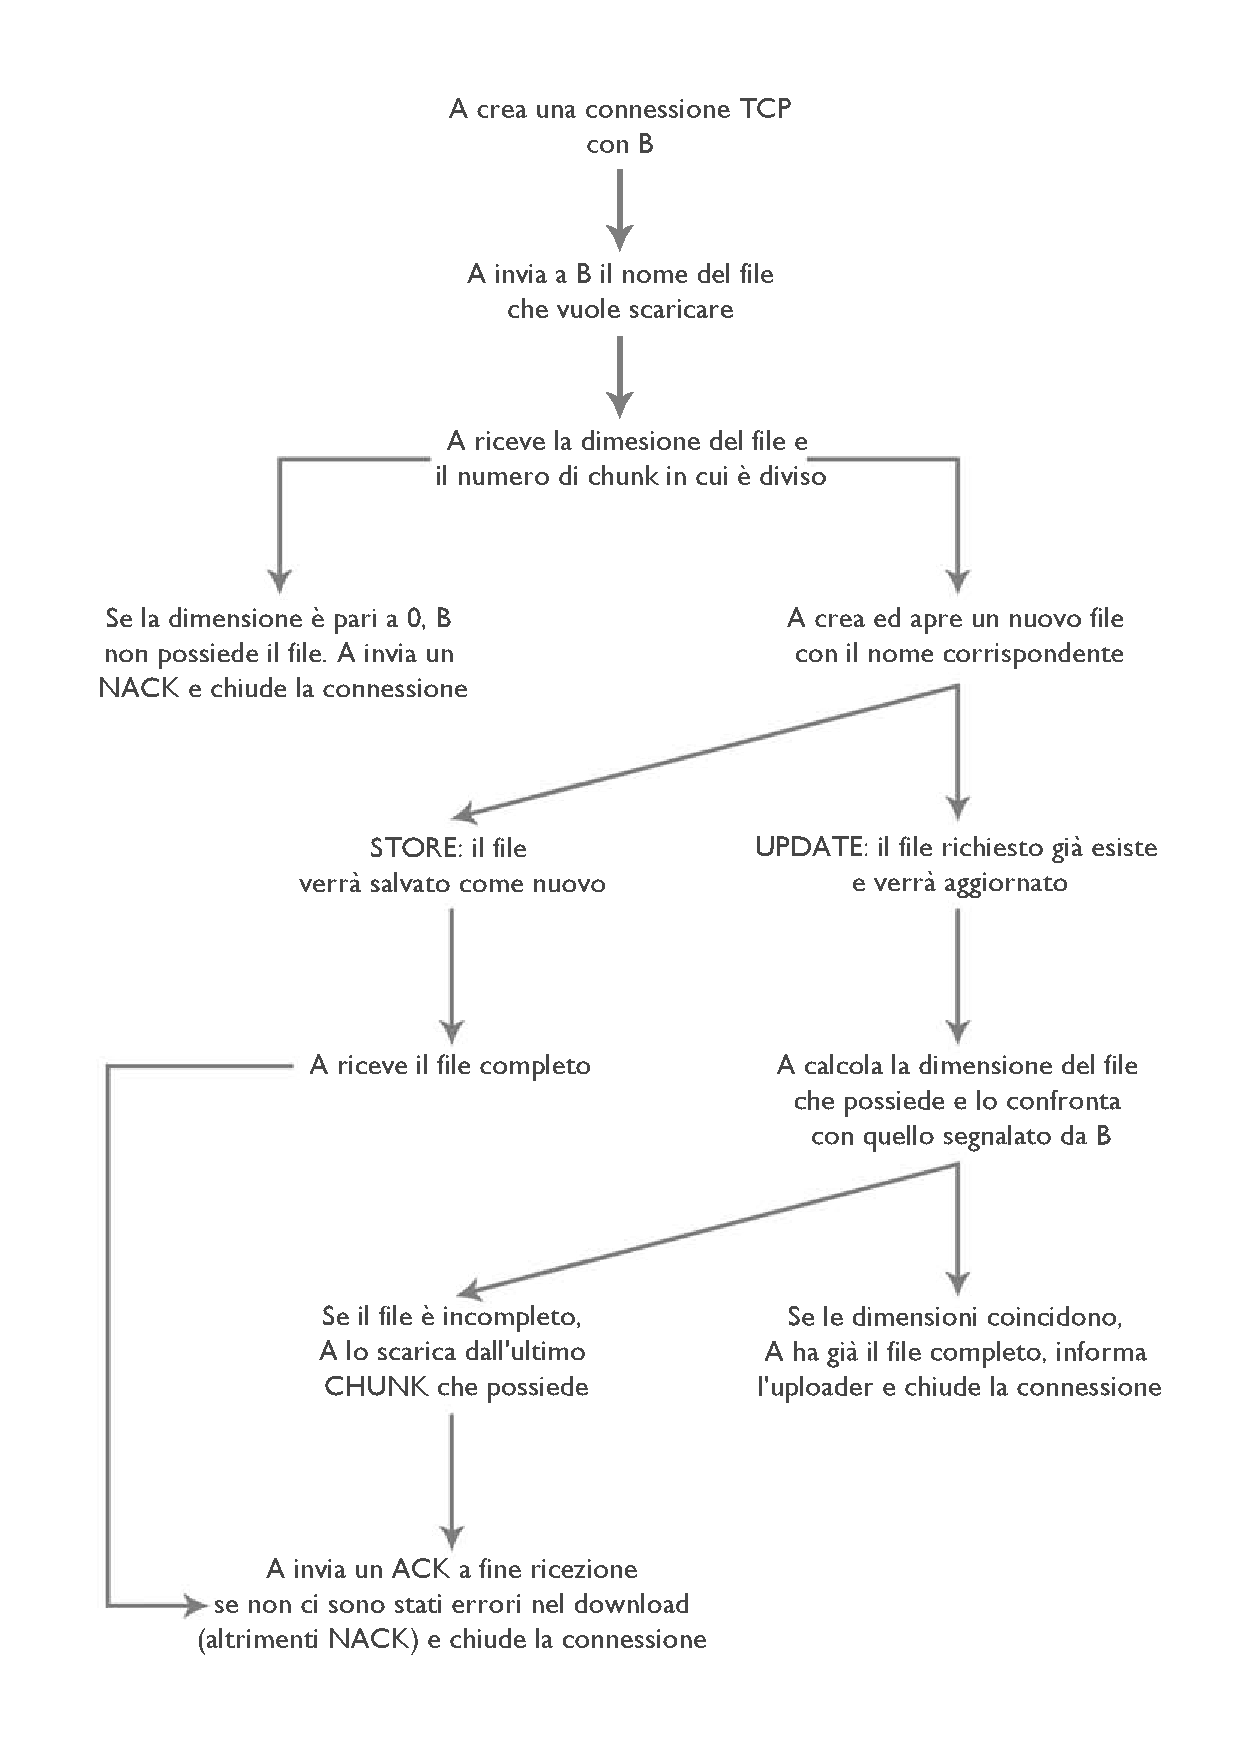
\includegraphics[width=12cm]{img/download}}
\caption{Esecuzione del download tra due peer\label{download_img}}
\end{figure}

\pagebreak

